% questions.tex —— 2008 年·普通高等学校招生考试·安徽卷·文科 · 题目内容片段（无答案）
% 由 tools/generate_projects.py 依来源总账自 2008/2008_数学真题_安徽文_试题.md 生成，勿手改（改源 MD 后重跑）


状态：needs-review；依固定候选 PDF 两页（印刷页 423–424）三栏图像以 300 dpi 渲染逐题核验，图形已矢量重绘，正式构建与逐页验收待完成。源未列各题分值，不补分值。

\gkpart{一、选择题}

\begin{question}
\gkti{1}若 $A$ 为全体实数的集合，$B=\{-2,-1,1,2\}$，则下列结论正确的是（　）

（A）$A\cap B=\{-2,-1\}$

（B）$(\complement_{\mathbf R}A)\cup B=(-\infty,0)$

（C）$A\cup B=(0,+\infty)$

（D）$(\complement_{\mathbf R}A)\cap B=\{-2,-1\}$

\end{question}
\begin{question}
\gkti{2}若 $\overrightarrow{AB}=(2,4)$，$\overrightarrow{AC}=(1,3)$，则 $\overrightarrow{BC}=$（　）

（A）$(1,1)$

（B）$(-1,-1)$

（C）$(3,7)$

（D）$(-3,-7)$

\end{question}
\begin{question}
\gkti{3}已知 $m$，$n$ 是两条不同直线，$\alpha$，$\beta$，$\gamma$ 是三个不同平面，下列命题中正确的是（　）

（A）若 $\alpha\perp\gamma$，$\beta\perp\gamma$，则 $\alpha\parallel\beta$

（B）若 $m\perp\alpha$，$n\perp\alpha$，则 $m\parallel n$

（C）若 $m\parallel\alpha$，$n\parallel\alpha$，则 $m\parallel n$

（D）若 $m\parallel\alpha$，$m\parallel\beta$，则 $\alpha\parallel\beta$

\end{question}
\begin{question}
\gkti{4}$a<0$ 是方程 $ax^2+1=0$ 有一个负数根的（　）

（A）必要不充分条件

（B）充分必要条件

（C）充分不必要条件

（D）既不充分也不必要条件

\end{question}
\begin{question}
\gkti{5}在三角形 $ABC$ 中，$AB=5$，$AC=3$，$BC=7$，则 $\angle BAC$ 的大小为（　）

（A）$\dfrac{2\pi}{3}$

（B）$\dfrac{5\pi}{6}$

（C）$\dfrac{3\pi}{4}$

（D）$\dfrac{\pi}{3}$

\end{question}
\begin{question}
\gkti{6}函数 $f(x)=(x-1)^2+1$（$x\leqslant0$）的反函数为（　）

（A）$f^{-1}(x)=1-\sqrt{x-1}$（$x\geqslant1$）

（B）$f^{-1}(x)=1+\sqrt{x-1}$（$x\geqslant1$）

（C）$f^{-1}(x)=1-\sqrt{x-1}$（$x\geqslant2$）

（D）$f^{-1}(x)=1-\sqrt{x-1}$（$x\geqslant2$）

\end{question}
\begin{question}
\gkti{7}设 $(1+x)^8=a_0+a_1x+\cdots+a_8x^8$，则 $a_0$，$a_1$，$\cdots$，$a_8$ 中奇数的个数为（　）

（A）$2$

（B）$3$

（C）$4$

（D）$5$

\end{question}
\begin{question}
\gkti{8}函数 $y=\sin\left(2x+\dfrac{\pi}{3}\right)$ 图象的对称轴方程可能是（　）

（A）$x=-\dfrac{\pi}{6}$

（B）$x=-\dfrac{\pi}{12}$

（C）$x=\dfrac{\pi}{6}$

（D）$x=\dfrac{\pi}{12}$

\end{question}
\begin{question}
\gkti{9}设函数 $f(x)=2x+\dfrac1x-1$（$x<0$），则 $f(x)$（　）

（A）有最大值

（B）有最小值

（C）是增函数

（D）是减函数

\end{question}
\begingroup
\renewenvironment{question}{\Needspace{0.46\textheight}}{}
\begin{question}
\gkti{10}若过点 $A(4,0)$ 的直线 $l$ 与曲线 $(x-2)^2+y^2=1$ 有公共点，则直线 $l$ 的斜率的取值范围为（　）

（A）$(-\sqrt3,\sqrt3)$

（B）$[-\sqrt3,\sqrt3]$

（C）$\left(-\dfrac{\sqrt3}{3},\dfrac{\sqrt3}{3}\right)$

（D）$\left[-\dfrac{\sqrt3}{3},\dfrac{\sqrt3}{3}\right]$

\end{question}
\endgroup
\begin{question}
\gkti{11}若 $A$ 为不等式组 $\begin{cases}x\leqslant0,\\ y\geqslant0,\\ y-x\leqslant2\end{cases}$ 表示的平面区域，则当 $a$ 从 $-2$ 连续变化到 $1$ 时，动直线 $x+y=a$ 扫过 $A$ 中的那部分区域的面积为（　）

（A）$\dfrac34$

（B）$1$

（C）$\dfrac74$

（D）$2$

\end{question}
\begin{question}
\gkti{12}$12$ 名同学合影，站成前排 $4$ 人后排 $8$ 人，现摄影师要从后排 $8$ 人中抽 $2$ 人调整到前排，若其他人的相对顺序不变，则不同调整方法的总数是（　）

（A）$\mathrm C_8^2\mathrm A_6^6$

（B）$\mathrm C_8^2\mathrm A_3^2$

（C）$\mathrm C_8^2\mathrm A_6^2$

（D）$\mathrm C_8^2\mathrm A_5^2$

\end{question}
\gkpart{二、填空题}

\begin{question}
\gkti{13}函数 $f(x)=\dfrac{\sqrt{|x-2|-1}}{\log_2(x-1)}$ 的定义域为\gkblank{}。

\end{question}
\begin{question}
\gkti{14}已知双曲线 $\dfrac{x^2}{n}-\dfrac{y^2}{12-n}=1$ 的离心率是 $\sqrt3$，则 $n=$\gkblank{}。

\end{question}
\begin{question}
\gkti{15}在数列 $\{a_n\}$ 中，$a_n=4n-\dfrac52$，$a_1+a_2+\cdots+a_n=an^2+bn$，$n\in\mathbf N^*$，其中 $a$，$b$ 为常数，则 $ab=$\gkblank{}。

\end{question}
\begin{question}
\gkti{16}已知 $A$，$B$，$C$，$D$ 在同一个球面上，$AB\perp$ 平面 $BCD$，$BC\perp CD$，若 $AB=6$，$AC=2\sqrt{13}$，$AD=8$，则 $B$，$C$ 两点间的球面距离是\gkblank{}。

\end{question}
\gkpart{三、解答题}

\begin{question}
\gkti{17}已知函数 $f(x)=\cos\left(2x-\dfrac{\pi}{3}\right)+2\sin\left(x-\dfrac{\pi}{4}\right)\sin\left(x+\dfrac{\pi}{4}\right)$。

（1）求函数 $f(x)$ 的最小正周期；

（2）求函数 $f(x)$ 在区间 $\left[-\dfrac{\pi}{12},\dfrac{\pi}{2}\right]$ 上的值域。

\end{question}
\begingroup
\renewenvironment{question}{\Needspace{0.46\textheight}}{}
\begin{question}
\gkti{18}在某次普通话测试中，为测试汉字发音水平，设置了 $10$ 张卡片，每张卡片印有一个汉字的拼音，其中恰有 $3$ 张卡片上的拼音带有后鼻音“g”。

（1）现对三位被测试者先后进行测试，第一位被测试者从这 $10$ 张卡片中随机抽取 $1$ 张，测试后放回，余下 $2$ 位的测试，也按同样的方法进行。求这三位被测试者抽取的卡片上，拼音都带有后鼻音“g”的概率；

（2）若某位被测试者从 $10$ 张卡片中一次随机抽取 $3$ 张，求这三张卡片上，拼音带有后鼻音“g”的卡片不少于 $2$ 张的概率。

\Needspace{0.4\textheight}
\end{question}
\endgroup
\begin{question}
\gkti{19}如图，在四棱锥 $O-ABCD$ 中，底面 $ABCD$ 是边长为 $1$ 的菱形，$\angle ABC=\dfrac{\pi}{4}$。$OA\perp$ 底面 $ABCD$，$OA=2$，$M$ 为 $OA$ 的中点。

（1）求异面直线 $AB$ 与 $MD$ 所成角的大小；

（2）求点 $B$ 到平面 $OCD$ 的距离。
\nopagebreak[4]
\begin{center}% 2008 年安徽卷文科第 19 题：四棱锥 O-ABCD，底面 ABCD 是边长为 1 的菱形，
%   ∠ABC=π/4，OA⊥底面 ABCD，OA=2，M 为 OA 的中点。
% 来源 PDF：gaokaomath-src/普通高考/2008/2008安徽文.pdf
% SHA-256：a7276afab60af4cf2bfc8265c3c7da749c4c7613cf5c5d30fe955007b545bb77
% 原页：2008安徽文.pdf 第 1 页（A3 三栏）第 3 栏，书页码 423。
% 重绘依据：按原页斜投影重绘：A 为被遮挡的后顶点，B 在左前、C 在右前、D 在右后，
%   A—B、A—D、A—O 用虚线，M 取 OA 中点并以虚线连 M—D。
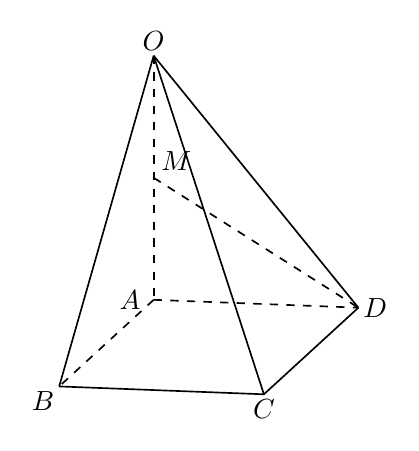
\begin{tikzpicture}[scale=1.0, semithick,
  every node/.style={inner sep=1.5pt}]

  \coordinate (B) at (0.60,1.00);
  \coordinate (C) at (3.20,0.90);
  \coordinate (D) at (4.40,2.00);
  \coordinate (A) at (1.80,2.10);
  \coordinate (O) at (1.80,5.20);
  \coordinate (M) at (1.80,3.65);

  % 底面：前棱与右棱可见，后两条棱被遮挡
  \draw (B) -- (C) -- (D);
  \draw[dashed] (A) -- (B);
  \draw[dashed] (A) -- (D);

  % 侧棱
  \draw (O) -- (B);
  \draw (O) -- (C);
  \draw (O) -- (D);
  \draw[dashed] (O) -- (A);

  % M 为 OA 中点，连 MD
  \draw[dashed] (M) -- (D);

  \node[above] at (O) {$O$};
  \node[above right=1pt] at (M) {$M$};
  \node[left=3pt] at (A) {$A$};
  \node[below left] at (B) {$B$};
  \node[below] at (C) {$C$};
  \node[right] at (D) {$D$};
\end{tikzpicture}
\end{center}
\nopagebreak[4]
\end{question}
\begin{question}
\gkti{20}设函数 $f(x)=\dfrac a3x^3-\dfrac32x^2+(a+1)x+1$，其中 $a$ 为实数。

（1）已知函数 $f(x)$ 在 $x=1$ 处取得极值，求 $a$ 的值；

（2）已知不等式 $f'(x)>x^2-x-a+1$ 对任意 $a\in(0,+\infty)$ 都成立，求实数 $x$ 的取值范围。

\end{question}
\begin{question}
\gkti{21}设数列 $\{a_n\}$ 满足 $a_1=a$，$a_{n+1}=ca_n+1-c$，$n\in\mathbf N^*$，其中 $a$，$c$ 为实数，且 $c\neq0$。

（1）求数列 $\{a_n\}$ 的通项公式；

（2）设 $a=\dfrac12$，$c=\dfrac12$，$b_n=n(1-a_n)$，$n\in\mathbf N^*$，求数列 $\{b_n\}$ 的前 $n$ 项和 $S_n$；

（3）若 $0<a_n<1$ 对任意 $n\in\mathbf N^*$ 成立，证明 $0<c\leqslant1$。

\end{question}
\begin{question}
\gkti{22}设椭圆 $C$：$\dfrac{x^2}{a^2}+\dfrac{y^2}{b^2}=1$（$a>b>0$）其相应于焦点 $F(2,0)$ 的准线方程为 $x=4$。

（1）求椭圆 $C$ 的方程；

（2）已知过点 $F_1(-2,0)$ 倾斜角为 $\theta$ 的直线交椭圆 $C$ 于 $A$，$B$ 两点，求证：$|AB|=\dfrac{4\sqrt2}{2-\cos^2\theta}$；

（3）过点 $F_1(-2,0)$ 作两条互相垂直的直线分别交椭圆 $C$ 于 $A$，$B$ 和 $D$，$E$，求 $|AB|+|DE|$ 的最小值。

\end{question}